%% GeneDiseaseTrace-LLM: manuscript for the Journal of Biomedical Informatics.
%% Layout and section logic follow a recent JBI paper prepared with elsarticle
%% (Park et al., "Automated Identification of Incidentalomas Requiring Follow-Up", arXiv:2512.05537).
%% Build: latexmk -pdf main.tex
\documentclass[preprint,10pt,letterpaper]{elsarticle}

\usepackage[T1]{fontenc}
\usepackage[utf8]{inputenc}
\usepackage{lmodern}
\usepackage[letterpaper,hmargin=1.35in,vmargin=1.1in]{geometry}   % text block of the model paper
\usepackage{microtype}
\usepackage{amsmath,amssymb}
\usepackage{booktabs,tabularx,multirow,array}
\usepackage{xcolor}
\usepackage{graphicx}
\usepackage[hidelinks]{hyperref}
\usepackage{enumitem}
\setlist{nosep}
\setlength{\emergencystretch}{3em}
\renewcommand{\topfraction}{0.9}
\renewcommand{\floatpagefraction}{0.8}
% Shared palette and TikZ/pgfplots settings for all figures (loaded by main.tex
% and graphical_abstract.tex). Colours are colour-blind safe (Okabe-Ito based).
\usepackage{tikz}
\usepackage{pgfplots}
\pgfplotsset{compat=1.18}
\usepgfplotslibrary{groupplots}
\usetikzlibrary{arrows.meta,positioning,fit,backgrounds,calc,shapes.misc,decorations.pathreplacing}

% Systems
\definecolor{ours}{HTML}{0B5CAD}      % our method (Claude Opus 5.5)
\definecolor{gpt}{HTML}{009E73}       % our method with GPT-6.1 Sol
\definecolor{pubtator}{HTML}{D55E00}  % PubTator3
% Entities
\definecolor{genefill}{HTML}{DCEBFA}
\definecolor{geneline}{HTML}{0B5CAD}
\definecolor{disfill}{HTML}{FBE3D6}
\definecolor{disline}{HTML}{C2410C}
% Statuses
\definecolor{stsup}{HTML}{1B7F4B}
\definecolor{stunc}{HTML}{B45309}
\definecolor{stneg}{HTML}{B4233C}
\definecolor{stnf}{HTML}{475569}
% Neutrals (all text uses dark ink; light tones are for borders/fills only)
\definecolor{ink}{HTML}{1F2933}
\definecolor{rule}{HTML}{CBD5E1}
\definecolor{panel}{HTML}{F8FAFC}

\tikzset{
  panel/.style={draw=rule, fill=panel, rounded corners=3pt, inner sep=6pt},
  paneltitle/.style={font=\sffamily\bfseries\small, text=ink, anchor=north west},
  gene/.style={fill=genefill, draw=geneline, text=ink, rounded corners=1.5pt, inner sep=1.6pt, font=\sffamily\scriptsize},
  dis/.style={fill=disfill, draw=disline, text=ink, rounded corners=1.5pt, inner sep=1.6pt, font=\sffamily\scriptsize},
  badge/.style={rounded corners=2pt, inner sep=1.8pt, font=\sffamily\tiny\bfseries, text=white},
  flow/.style={-{Stealth[length=2.2mm]}, line width=0.9pt, draw=ink},
}
% Inline highlights inside text nodes
\newcommand{\hlgene}[1]{\tikz[baseline=(g.base)]\node[fill=genefill, inner sep=0.6pt, rounded corners=1pt] (g) {\strut #1};}
\newcommand{\hldis}[1]{\tikz[baseline=(d.base)]\node[fill=disfill, inner sep=0.6pt, rounded corners=1pt] (d) {\strut #1};}
\newcommand{\sid}[1]{{\ttfamily\color{ink}\tiny[#1]}}
\newcommand{\badge}[2]{\tikz[baseline=(b.base)]\node[badge, fill=#1] (b) {#2};}

\pgfplotsset{
  gdt/.style={
    font=\sffamily\scriptsize,
    tick label style={font=\sffamily\tiny, text=ink},
    label style={font=\sffamily\scriptsize, text=ink},
    title style={font=\sffamily\bfseries\scriptsize, text=ink, align=center},
    axis line style={draw=ink},
    tick style={draw=ink},
    major grid style={draw=rule, line width=0.3pt},
    grid=major,
  },
}


\newcommand{\st}[1]{\texttt{#1}}             % status and reason-code names
\newcommand{\todo}[1]{\textcolor{stneg}{[TODO: #1]}}

\journal{Journal of Biomedical Informatics}

\begin{document}

\begin{frontmatter}

\title{Prompt Rules, Input Scope, and Selective Annotation in Zero-Shot Gene--Disease Relation Extraction: A Controlled Multi-Benchmark Evaluation of Large Language Models}

\author[a]{Zeqian Tong}
\author[b]{\todo{co-authors}}
\affiliation[a]{organization={\todo{affiliation}}}
\affiliation[b]{organization={\todo{affiliation}}}

\begin{abstract}
\setlength{\parindent}{0pt}\setlength{\parskip}{6pt}%
\textbf{Objective:} Public gene--disease resources such as PubTator3 derive relations from abstracts and return pairs without evidence sentences, certainty grades, or study-versus-background provenance. We evaluated what a zero-shot large language model (LLM) pipeline that emits this curation schema can and cannot deliver on abstracts and full texts, and how specific prompt versions and input scope changed its results.

\textbf{Methods:} Using one extraction request per paper (and at most one repair request on validation failure), an LLM follows a 108-word task prompt and cites sentences by ID; a deterministic validator checks that every entity mention occurs verbatim and that every cited sentence ID resolves. We compared this minimal prompt with a 1,045-word decision card, and compared both with PubTator3 on BioRED, EU-ADR, and RENET2. On BioTriplex, a manually annotated full-text corpus (30 articles locked before any run), we compared abstract and full-text input for the same system, a second LLM, and two supervised models run locally: BioREx, the relation model inside PubTator3, applied over paragraphs, and the released RENET2 models trained on full text. We repeated the Claude and supervised comparisons on 49 further BioTriplex articles under a protocol written before the run. All systems were scored with one-to-one matching and paired bootstrap intervals.

\textbf{Results:} The decision card lowered F1 on BioRED (0.551 vs 0.665 on Dev+Test) by lowering recall (0.418 vs 0.604). On BioRED Test and on BioTriplex abstracts, the minimal prompt and PubTator3 were not distinguishable (F1 0.614 vs 0.680; 0.395 vs 0.377). Reading the full text raised recall on BioTriplex from 0.366 to 0.813 for Claude Opus 5.5, from 0.302 to 0.884 for GPT-6.1 Sol, and from 0.291 to 0.722 for BioREx; RENET2 changed less (0.245 to 0.344, interval spanning zero). On articles with valid LLM output (Claude 25 of 30, GPT 27 of 30), the LLMs had higher F1 than abstract-trained BioREx (0.525 vs 0.332; 0.433 vs 0.304) through higher precision, and annotation-category counts place most of that difference in entity scope and duplicate pairs. Against full-text-trained RENET2, Claude had similar precision and higher recall (0.813 vs 0.366), and the F1 differences for both LLMs had intervals spanning zero. In a stratified single-annotator check, cited sentences alone were judged sufficient for 58.5\% of supported pairs on BioRED and 75.4\% on BioTriplex; 5.6\% on each corpus were judged unsupported. On the 49 further articles, with failed articles counted as empty answers, the prespecified comparison confirmed the recall gain from full text for Claude (+0.322); among articles with valid output, F1 exceeded RENET2 (0.474 vs 0.212). Full-text extraction cost about USD 0.40 per article; safety filters left 13\% of locked and 29\% of further BioTriplex full texts without a result for the primary model.

\textbf{Conclusion:} On BioTriplex, reading the full text raised recall for the LLMs and BioREx; on BioRED abstracts, one detailed decision card lowered recall, an ablation of that card and not a general result about rules. Zero-shot LLMs performed in the range of supervised abstract-level extraction. On full text their recall was similar to BioREx and higher than RENET2, but F1 comparisons depended on entity scope, training text, and a selective gold standard, so they should not be read as better relation judgment. All citations resolved, yet in a single-annotator check they were sufficient on their own for only part of the supported pairs, so they point curators to evidence and should be read with the surrounding text. Safety-filter failures were frequent enough to change deployment recall, so a full-text pipeline needs a fallback.
\end{abstract}

\begin{keyword}
Relation Extraction; Gene--Disease Association; Large Language Models; Full-Text Mining; Biocuration; Evaluation Methodology
\end{keyword}

\end{frontmatter}

%% ===================================================================
\section{Introduction}

Curated gene--disease knowledge bases depend on continuous extraction from primary literature. Associations between genes and diseases underpin variant interpretation, drug-target discovery, and repositories such as DisGeNET~\cite{pinero2020disgenet} and CTD~\cite{davis2023ctd}. More than a million biomedical articles appear each year, so manual curation alone cannot keep pace. Supervised encoders~\cite{lee2020biobert,gu2021pubmedbert,lai2023biorex} and literature-scale systems such as PubTator3~\cite{wei2024pubtator3} achieve high F1 on benchmarks such as BioRED~\cite{luo2022biored} within their training domain.

Benchmark extraction and practical curation differ in output structure and text scope. Widely used public resources such as PubTator3 return positive pairs derived from abstracts, whereas curators need auditable records across the paper: verbatim supporting sentences, a distinction between demonstrated, hedged, and null findings, and a separation of a study's own results from background citations. On BioTriplex~\cite{collins2026biotriplex}, a manually annotated full-text corpus, 115 of the 151 relations in our evaluation set are linked only outside the abstract.

Large language models can read full papers and emit this schema, yet three questions remain open. First, curation-oriented prompting often relies on detailed rules, yet guideline-conditioned extraction~\cite{sainz2024gollie} and template-based systems~\cite{caufield2024spires} seldom report what a specific rule document costs in recall. Second, comparisons between full-text LLM extractors and abstract-level resources confound the method with the input. Third, gold standards are often selective, so unannotated valid relations are scored as false positives alongside genuine errors~\cite{wadhwa2023revisiting,fan2024evaluating}, and position-based scoring can credit one gold relation several times.

We address these questions with a controlled evaluation of one pipeline. The pipeline makes one extraction request per paper (with at most one repair request on validation failure), cites sentences by ID, and passes a deterministic validator. Around it we compare a minimal task prompt with a detailed decision card and with guideline-derived rules; evaluate on BioRED, EU-ADR, RENET2, and a locked BioTriplex set; separate input scope from method by running each system on abstracts and on full texts, including BioREx~\cite{lai2023biorex} over full-text paragraphs and the released full-text models of RENET2~\cite{su2021renet2}; replicate with a second LLM; score all systems with one-to-one matching; examine disagreements with exploratory blinded checks; and test whether cited sentences suffice as evidence. The contribution is empirical: the recall cost of one detailed decision card, the effect of input scope on coverage, and the way selective annotation and entity scope change system comparisons.

%% ===================================================================
\section{Related Work}

\subsection{Supervised Biomedical Relation Extraction}
Supervised domain encoders remain the primary baseline for biomedical relation extraction. BioBERT~\cite{lee2020biobert} and PubMedBERT~\cite{gu2021pubmedbert} fine-tune pretrained representations on annotated corpora; BioREx~\cite{lai2023biorex} pools heterogeneous datasets, and later work adds relation directionality~\cite{lai2025directionality}. PubTator3~\cite{wei2024pubtator3} deploys BioREx with entity recognition and normalization across PubMed and PMC and is the standard public resource and our primary comparator. In our checks its relation predictions were the same with and without its full-text export, so the behaviour of this model family on full-text paragraphs has not been characterized. Supervised full-text models are rare because full-text annotation is costly; RENET2~\cite{su2021renet2} is the main example for gene--disease relations, trained on released texts that cover the title, abstract, and early body, with labels built by iterative expansion. We run both BioREx and RENET2 on the same full-text set.

\subsection{Large Language Models for Relation Extraction and Biocuration}
Direct prompting of LLMs has generally trailed supervised encoders on biomedical relation extraction~\cite{chen2025benchmarking,islamaj2024biocreative,brokman2025benchmark,gade2025benchmarking}. Three lines of work combine LLMs with structure. Guideline-conditioned models such as GoLLIE~\cite{sainz2024gollie} and curation frameworks such as SPIRES~\cite{caufield2024spires} and DRAGON-AI~\cite{toro2024dragonai} supply schemas or rules. Cascades such as CoRE~\cite{song2026core} route low-confidence predictions of a supervised model to an LLM with retrieved examples, improving BioRED F1 with entity pairs given. Statement validation against supplied text~\cite{adam2025traceable} verifies given claims and reported 0.88 precision and 0.44 recall on BioRED-derived statements with corrupted negatives. Full-text evaluations on human genetics articles~\cite{yin2026benchmarking} and on BioTriplex~\cite{collins2026biotriplex} extend the scope beyond abstracts. We do not propose a new extraction algorithm; we measure, under one scorer, how specific prompt versions, input scope, and model family change end-to-end extraction results with deterministically resolved citations.

\subsection{Gene--Disease Benchmarks and Incomplete Gold Standards}
Public gene--disease benchmarks encode different annotation protocols and completeness assumptions. BioRED~\cite{luo2022biored} labels relations between concept pairs in 600 abstracts and marks primary findings as \emph{Novel}. EU-ADR~\cite{vanmulligen2012euadr} assigns consensus positive, speculative, or negative labels, where re-annotation has shown that guideline boundaries drive disagreement~\cite{li2015crowdsourcing}. RENET2~\cite{su2021renet2} restricts human review to tool-proposed candidates and assigns negatives automatically. BioTriplex~\cite{collins2026biotriplex} annotates relation phrases with gene and disease links across 100 full texts; its released BERT training scripts classify relation types without negative samples, so those supervised results do not measure end-to-end detection as defined here. When generative extractors are scored against such corpora, benchmark precision mixes factual errors with valid unannotated relations~\cite{wadhwa2023revisiting,fan2024evaluating}. We therefore decompose apparent false positives by external annotation category and check samples of them blind.

%% ===================================================================
\section{Methods}

\subsection{Datasets}
Four public benchmarks with distinct annotation protocols evaluate the pipeline on abstracts and full texts (Table~\ref{tab:benchmarks}).

\subsubsection{BioRED}
A pair counts as a gold relation when one concept is a gene or gene product and the other a disease or phenotypic feature, pooled across relation subtypes. Prompt comparisons used the abstracts with at least one gene--disease relation in Dev (71) and Test (73). Test results additionally include the 27 Test abstracts without such a relation, where any \st{supported} pair counts as a false positive, giving all 100 Test abstracts. We selected the minimal prompt after inspecting Test results, so BioRED results are not a clean held-out estimate for it; BioTriplex serves that role.

\subsubsection{EU-ADR}
We used all 100 abstracts of the EU-ADR target--disorder subset, comprising 134 consensus pairs: 122 positive (PA), 9 speculative (SA), and 3 negative (NA). Precision and recall treat PA pairs as gold positives; SA and NA pairs evaluate the non-binary statuses.

\subsubsection{RENET2}
We drew 40 full-text articles from RENET2 (seed 20261028), whose released texts cover the title, abstract, and early body. The sample contains 181 associated, 83 non-associated, and 1 ambiguous pair; non-associated labels were assigned by text-mining tools without manual verification.

\subsubsection{BioTriplex}
BioTriplex~\cite{collins2026biotriplex} contains 100 PMC open-access articles split by article into train (70), validation (15), and test (15), with gene and disease mentions, relation phrases, links, and a background or result location for each relation. None of the 100 articles occurs in BioRED, RENET2, EU-ADR, or our development papers (checked by PMID). Because our system is zero-shot, we locked validation plus test (30 articles) as the evaluation set before any run; five train articles were used only to check the adaptation. Entities carry no database identifiers, so we merged mentions of one type within an article by normalized text and by adjacent ``long form (short form)'' patterns. A gene--disease pair is a gold relation when at least one link carries a relation other than \emph{no relation}, collapsing the 21 types. The set contains 151 gold relations in 21 articles: 36 linked in the abstract and 115 linked only outside it. The corpus authors report 0.71 F1 agreement on relation annotation~\cite{collins2026biotriplex}. A second validation batch comprises all 49 remaining train articles with relation links (329 gold relations, 254 linked only outside the abstract), prepared with the same rules. No system was trained or tuned on them, but they were chosen after the locked results were known, so we treat them as further validation and report them separately.

\begin{table}[!htbp]
\centering\footnotesize
\caption{\textbf{Public gene--disease benchmarks evaluated in this study.} The four corpora span PubMed abstracts and PMC full texts under different annotation scopes and negative-label protocols.}
\label{tab:benchmarks}
\begin{tabularx}{\linewidth}{@{}l>{\raggedright\arraybackslash}p{2.2cm}>{\raggedright\arraybackslash}X>{\raggedright\arraybackslash}p{3.3cm}>{\raggedright\arraybackslash}p{2.5cm}@{}}
\toprule
Benchmark & Text & Documents used & Gold gene--disease relations & Labels beyond ``related''\\
\midrule
BioRED~\cite{luo2022biored} & PubMed abstracts & Dev 71; Test 100 (73 with a relation) & 293 Dev; 295 Test & Novel / not novel\\
EU-ADR~\cite{vanmulligen2012euadr} & PubMed abstracts & Target--disorder subset, 100 abstracts & 134 consensus pairs: 122 PA, 9 SA, 3 NA & Positive / speculative / negative\\
RENET2~\cite{su2021renet2} & PMC text (title, abstract, early body) & Random sample of 40 articles & 181 associated; 83 non-associated; 1 ambiguous & Negatives tool-assigned\\
BioTriplex~\cite{collins2026biotriplex} & PMC full text by subsection & Locked set of 30 articles (validation + test) & 151 relations; 115 only outside the abstract & Background / result; 21 types\\
\bottomrule
\end{tabularx}
\end{table}

\subsection{Extraction Pipeline}

\subsubsection{Task Definition}
Given one paper as plain text, the extractor identifies gene and disease entities, links each entity to its verbatim surface forms, and assigns one of four mutually exclusive statuses to every gene $\times$ disease pair (Table~\ref{tab:status}). Every \st{supported} pair also receives a relation type (causal, correlation, or association), a source label (this study, background, both, or unclear), and cited sentence IDs.

\begin{table}[!htbp]
\centering\footnotesize
\caption{\textbf{Four-way pair status schema assigned to every extracted gene $\times$ disease pair.} Only \st{supported} pairs count as positive predictions under the default strict view.}
\label{tab:status}
\begin{tabularx}{\linewidth}{@{}lX@{}}
\toprule
Status & Definition in the minimal prompt\\
\midrule
\textcolor{stsup}{\st{supported}} & The paper gives evidence of a relationship.\\
\textcolor{stunc}{\st{uncertain}} & There is some evidence, but it is not conclusive. A reason code is required.\\
\textcolor{stneg}{\st{explicit\_negative}} & The paper reports that there is no relationship.\\
\textcolor{ink}{\st{not\_found}} & No evidence; includes unlisted pairs. It does not mean the pair is medically unrelated.\\
\bottomrule
\end{tabularx}
\end{table}

\subsubsection{Processing Steps}
Every paper passes through four sequential steps: deterministic packing, language-model generation, deterministic expansion, and schema validation (Fig.~\ref{fig:pipeline}). \emph{Packing} splits the document into numbered blocks and sentences with stable IDs and strips references and administrative sections. \emph{Generation} makes one extraction request (medium reasoning effort, all tools disabled) that emits pipe-separated lines; the model cites sentences by ID only, preventing altered quotations. \emph{Expansion} matches surface forms verbatim, resolves sentence IDs to quotes and offsets, and fills unlisted pairs as \st{not\_found}. \emph{Validation} checks these properties and the schema; any error triggers at most one repair request listing the violations. The validator verifies only that every entity surface form occurs verbatim and that every cited sentence ID resolves to a source sentence. Whether a cited sentence supports a relation remains the model's judgment and is not checked by the pipeline; we examined it separately with a single-annotator check of a stratified sample (Section~\ref{sec:checks}). Fig.~\ref{fig:example} illustrates the output.

\begin{figure}[!htbp]
\centering
\resizebox{\linewidth}{!}{% Figure 1 in the manuscript. Four-step extraction pipeline with concise keyword nodes and dark ink text.
\newcommand{\stagebox}[2]{\begin{minipage}[t][2.25cm][t]{#1}\raggedright #2\end{minipage}}
\newcommand{\codeline}{\ttfamily\fontsize{6.4pt}{7.6pt}\selectfont\color{ink}}
\begin{tikzpicture}[
  font=\sffamily\scriptsize, text=ink,
  every node/.append style={execute at begin node={\hyphenpenalty=10000\exhyphenpenalty=10000}},
  stage/.style={draw=rule, fill=panel, rounded corners=3pt, align=left, inner sep=4.5pt, anchor=north west},
  llm/.style={stage, draw=ours, fill=genefill, line width=0.8pt},
  io/.style={draw=rule, fill=white, rounded corners=2pt, text width=1.85cm, align=left, inner sep=3.5pt},
  note/.style={font=\sffamily\scriptsize, text=ink},
]
% Steps (top-aligned, equal height, keyword-only)
\node[stage] (pack) at (2.75,0) {\stagebox{2.2cm}{%
  {\bfseries 1\enspace Packing}\par\smallskip
  Assign sentence IDs\par
  Drop references\par
  Cache system prompt\par\smallskip
  {\codeline b0098.s12}}};
\node[llm] (gen) at ($(pack.north east)+(0.45,0)$) {\stagebox{2.65cm}{%
  {\bfseries\color{ours} 2\enspace LLM Generation}\par\smallskip
  One extraction call\par
  Cite sentence IDs only\par\smallskip
  {\codeline E|G5|gene|MAP3K3|...\\EV|V7|b0098.s12|...\\P|G5|D3|sup|a|bg|...}}};
\node[stage] (exp) at ($(gen.north east)+(0.45,0)$) {\stagebox{2.2cm}{%
  {\bfseries 3\enspace Expansion}\par\smallskip
  Match surface forms\par
  Resolve quotes \& offsets\par
  Fill gene $\times$ disease matrix}};
\node[stage] (val) at ($(exp.north east)+(0.45,0)$) {\stagebox{2.2cm}{%
  {\bfseries 4\enspace Validation}\par\smallskip
  Verify verbatim spans\par
  Verify sentence IDs\par
  Check schema \& reasons}};
% Inputs and output, centred on the step row
\path (pack.west) ++(-0.45,0) coordinate (inmid);
\node[io, anchor=south east] (paper) at ($(inmid)+(0,0.08)$) {\textbf{Paper}\\Full text or abstract};
\node[io, anchor=north east] (card) at ($(inmid)+(0,-0.08)$) {\textbf{Decision card}\\Frozen rules + schema};
\node[io, anchor=west] (out) at ($(val.east)+(0.6,0)$) {\textbf{Output}\\Entities \& mentions\\Evidence quotes\\4-status pair matrix};
% Arrows
\draw[flow] (paper.east) -- ++(0.2,0) |- ([yshift=3pt]pack.west);
\draw[flow] (card.east) -- ++(0.2,0) |- ([yshift=-3pt]pack.west);
\draw[flow] (pack) -- (gen);
\draw[flow] (gen) -- (exp);
\draw[flow] (exp) -- (val);
\draw[flow, draw=stsup] (val) -- node[above, note, text=stsup, font=\sffamily\scriptsize\bfseries] {pass} (out);
% Repair loop below the row
\draw[flow, draw=stneg, densely dashed, line width=1pt] (val.south) -- ++(0,-0.42) -| (gen.south);
\node[note, text=stneg, anchor=north, align=center] (fail) at ($(gen.south)!0.5!(val.south)+(0,-0.48)$)
  {\textbf{fail} $\rightarrow$ at most 1 repair request with error list};
% Legend on the left
\node[note, anchor=north west, text=ink] (leg) at ($(card.west |- fail.south)+(0,0.18)$)
  {\textcolor{ours}{\rule{7pt}{7pt}}\,LLM call\quad \textcolor{rule!80!black}{\rule{7pt}{7pt}}\,Deterministic code};
\end{tikzpicture}
}
\caption{\textbf{Architecture of the four-step extraction pipeline.} Steps~1, 3, and~4 execute deterministic code; Step~2 makes one extraction request to the language model. Any output that fails verbatim surface-form, sentence-ID, or schema checks in Step~4 triggers at most one repair request listing the validation errors.}
\label{fig:pipeline}
\end{figure}

\begin{figure}[!htbp]
\centering
\resizebox{\linewidth}{!}{% Figure 2. Worked example: PMC10014009 (Kim et al., 2023; CC BY-NC-ND 4.0, short quotes).
\newcommand{\fG}[1]{{\setlength{\fboxsep}{0.8pt}\colorbox{genefill}{\strut\textcolor{geneline!85!black}{#1}}}}
\newcommand{\fD}[1]{{\setlength{\fboxsep}{0.8pt}\colorbox{disfill}{\strut\textcolor{disline!85!black}{#1}}}}
\newcommand{\fS}[1]{\leavevmode{\ttfamily\tiny\color{ink}#1}}
\newcommand{\fst}[2]{\leavevmode{\setlength{\fboxsep}{1.2pt}\colorbox{#1}{\textcolor{white}{\sffamily\tiny\bfseries #2}}}}
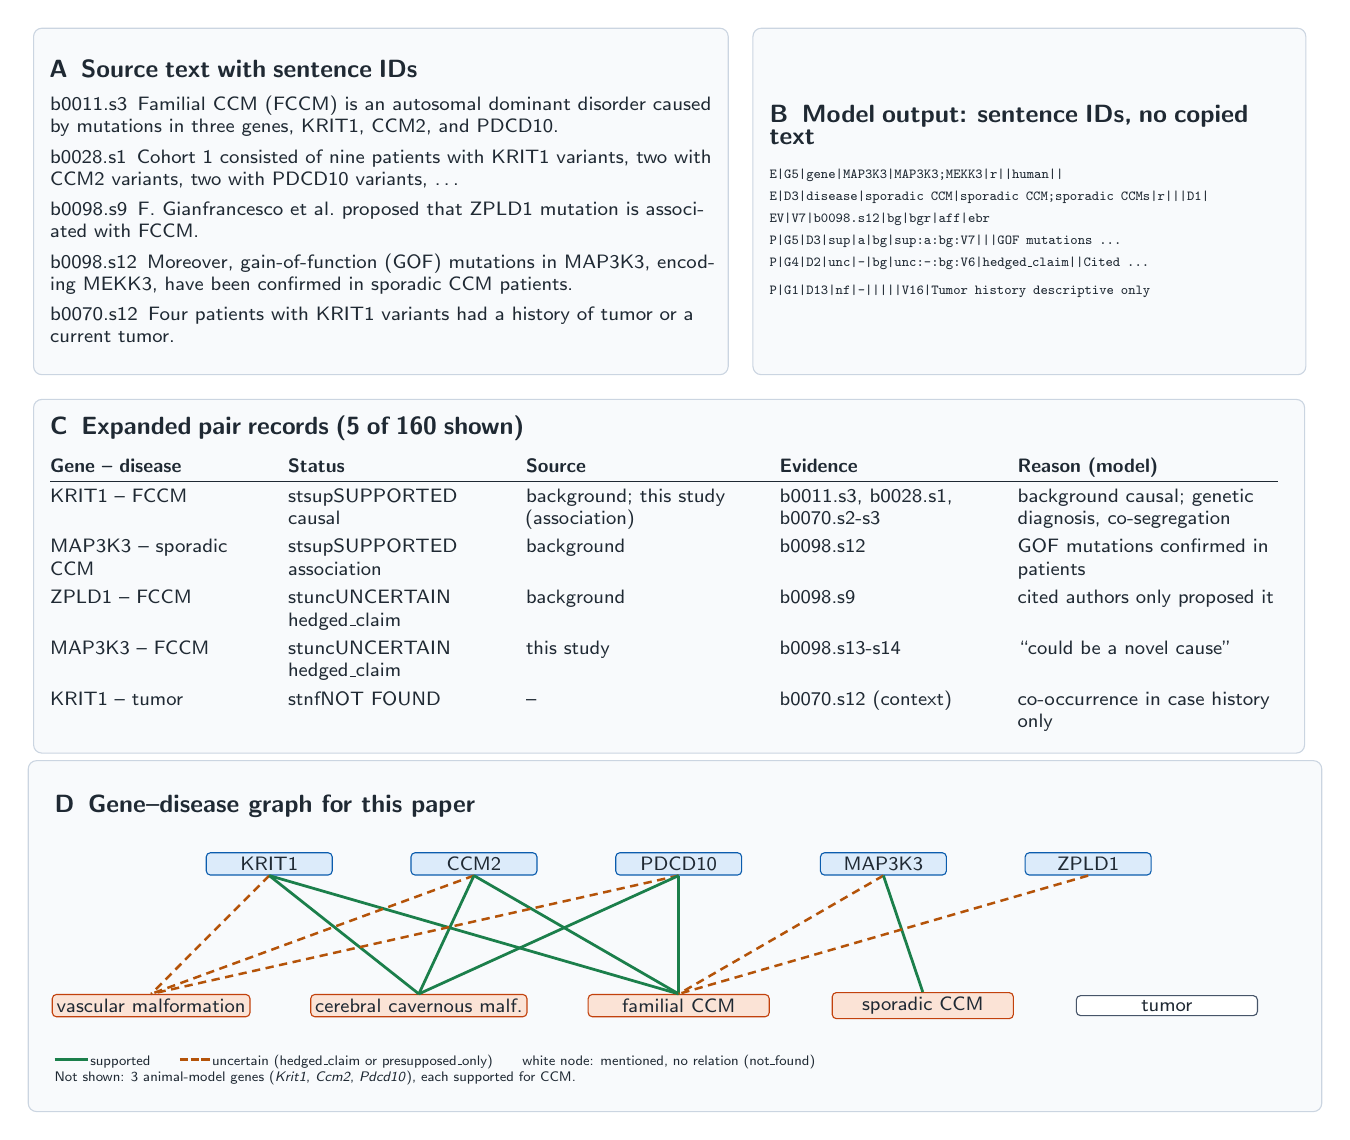
\begin{tikzpicture}[font=\sffamily\scriptsize, text=ink]
% ---------------- Panel A: source text
\node[panel, text width=8.4cm, minimum height=4.4cm, align=left, anchor=north west] (A) at (0,0) {%
  {\sffamily\bfseries\small A\enspace Source text with sentence IDs}\\[4pt]
  \fS{b0011.s3}\enspace \fD{Familial CCM (FCCM)} is an autosomal dominant disorder caused by mutations in three genes, \fG{KRIT1}, \fG{CCM2}, and \fG{PDCD10}.\\[3pt]
  \fS{b0028.s1}\enspace Cohort 1 consisted of nine patients with \fG{KRIT1} variants, two with \fG{CCM2} variants, two with \fG{PDCD10} variants, \dots\\[3pt]
  \fS{b0098.s9}\enspace F. Gianfrancesco et al.\ proposed that \fG{ZPLD1} mutation is associated with \fD{FCCM}.\\[3pt]
  \fS{b0098.s12}\enspace Moreover, gain-of-function (GOF) mutations in \fG{MAP3K3}, encoding \fG{MEKK3}, have been confirmed in \fD{sporadic CCM} patients.\\[3pt]
  \fS{b0070.s12}\enspace Four patients with \fG{KRIT1} variants had a history of \fD{tumor} or a current \fD{tumor}.};
% ---------------- Panel B: model output
\node[panel, text width=6.6cm, minimum height=4.4cm, align=left, anchor=north west] (B) at ($(A.north east)+(0.3,0)$) {%
  {\sffamily\bfseries\small B\enspace Model output: sentence IDs, no copied text}\\[6pt]
  {\ttfamily\tiny\color{ink}%
  E|G5|gene|MAP3K3|MAP3K3;MEKK3|r||human||\\[2pt]
  E|D3|disease|sporadic CCM|sporadic CCM;sporadic CCMs|r|||D1|\\[2pt]
  EV|V7|b0098.s12|bg|bgr|aff|ebr\\[2pt]
  P|G5|D3|sup|a|bg|sup:a:bg:V7|||GOF mutations ...\\[2pt]
  P|G4|D2|unc|-|bg|unc:-:bg:V6|hedged\_claim||Cited ...\\[2pt]
  P|G1|D13|nf|-|||||V16|Tumor history descriptive only}};
% ---------------- Panel C: expanded pair table (spans both columns)
\path (A.south west) ++(0,-0.3) coordinate (Cnw);
\path (B.east) coordinate (Bx);
\node[panel, text width=15.72cm, align=left, anchor=north west] (C) at (Cnw) {%
  {\sffamily\bfseries\small C\enspace Expanded pair records (5 of 160 shown)}\\[3pt]
  \renewcommand{\arraystretch}{1.3}%
  \begin{tabular}{@{}p{2.6cm}p{2.6cm}p{2.8cm}p{2.6cm}p{3.3cm}@{}}
  \textbf{Gene -- disease} & \textbf{Status} & \textbf{Source} & \textbf{Evidence} & \textbf{Reason (model)}\\\hline
  \fG{KRIT1} -- \fD{FCCM} & \fst{stsup}{SUPPORTED} causal & background; this study (association) & \fS{b0011.s3, b0028.s1, b0070.s2-s3} & background causal; genetic diagnosis, co-segregation\\
  \fG{MAP3K3} -- \fD{sporadic CCM} & \fst{stsup}{SUPPORTED} association & background & \fS{b0098.s12} & GOF mutations confirmed in patients\\
  \fG{ZPLD1} -- \fD{FCCM} & \fst{stunc}{UNCERTAIN} hedged\_claim & background & \fS{b0098.s9} & cited authors only proposed it\\
  \fG{MAP3K3} -- \fD{FCCM} & \fst{stunc}{UNCERTAIN} hedged\_claim & this study & \fS{b0098.s13-s14} & ``could be a novel cause''\\
  \fG{KRIT1} -- \fD{tumor} & \fst{stnf}{NOT FOUND} & -- & \fS{b0070.s12} (context) & co-occurrence in case history only\\
  \end{tabular}};
% ---------------- Panel D: per-paper bipartite graph (human genes; 3 animal-model genes omitted)
\begin{scope}[shift={($(C.south west)+(0,-0.3)$)},
  gnode/.style={gene, minimum width=1.6cm, font=\sffamily\scriptsize},
  dnode/.style={dis, minimum width=2.3cm, font=\sffamily\scriptsize},
  sup/.style={draw=stsup, line width=1pt},
  unc/.style={draw=stunc, line width=0.9pt, densely dashed}]
\node[anchor=north west, font=\sffamily\bfseries\small] (Dt) at (0.15,-0.1) {D\enspace Gene--disease graph for this paper};
\foreach \g/\x in {KRIT1/3.0, CCM2/5.6, PDCD10/8.2, MAP3K3/10.8, ZPLD1/13.4}
  \node[gnode] (g-\g) at (\x,-1.1) {\g};
\node[dnode] (d-VM) at (1.5,-2.9) {vascular malformation};
\node[dnode] (d-CCM) at (4.9,-2.9) {cerebral cavernous malf.};
\node[dnode] (d-FCCM) at (8.2,-2.9) {familial CCM};
\node[dnode] (d-SCCM) at (11.3,-2.9) {sporadic CCM};
\node[dnode, fill=white, draw=stnf, text=ink] (d-TUM) at (14.4,-2.9) {tumor};
\foreach \g in {KRIT1, CCM2, PDCD10} {
  \draw[unc] (g-\g.south) -- (d-VM.north);
  \draw[sup] (g-\g.south) -- (d-CCM.north);
  \draw[sup] (g-\g.south) -- (d-FCCM.north);
}
\draw[unc] (g-MAP3K3.south) -- (d-FCCM.north);
\draw[sup] (g-MAP3K3.south) -- (d-SCCM.north);
\draw[unc] (g-ZPLD1.south) -- (d-FCCM.north);
\node[anchor=north west, font=\sffamily\tiny, text=ink, align=left] (Dleg) at (0.15,-3.4)
  {\textcolor{stsup}{\rule[1.5pt]{12pt}{1pt}}\,supported\qquad
   \textcolor{stunc}{\rule[1.5pt]{3pt}{0.9pt}\,\rule[1.5pt]{3pt}{0.9pt}\,\rule[1.5pt]{3pt}{0.9pt}}\,uncertain (hedged\_claim or presupposed\_only)\qquad
   white node: mentioned, no relation (not\_found)\\
   Not shown: 3 animal-model genes (\textit{Krit1}, \textit{Ccm2}, \textit{Pdcd10}), each supported for CCM.};
\end{scope}
\begin{scope}[on background layer]
  \node[panel, fit={(Dt) (Dleg) (d-TUM) ($(C.south east)+(0,-0.3)$)}] {};
\end{scope}
\end{tikzpicture}
}
\caption{\textbf{Traceable output format on one full-text article, PMC10014009~\cite{kim2023fccm}.} (A)~Source excerpts with stable sentence IDs; gene mentions are highlighted in blue and disease mentions in coral. (B)~Compact pipe-separated model output citing sentence IDs only. (C)~Deterministically expanded pair records spanning three statuses and both provenance sources. (D)~Resulting document-level gene--disease graph. The example was produced with the decision card; all prompt variants share this output format. Excerpts are reproduced from an open-access article (CC~BY-NC-ND~4.0).}
\label{fig:example}
\end{figure}

\subsubsection{Prompt Variants}
All variants share a 595-word output format specification, the packed text, the validator, and model settings; they differ only in the task text. The shared specification itself carries instructions, so no variant is rule-free. The \emph{minimal prompt} is a 108-word task statement that lists the four statuses and asks for relation type, source, and sentence IDs; it is the default system in this paper. The \emph{decision card} is a 1,045-word rule document distilled from a longer guideline written on pilot articles. It adds entity-scope rules (general symptoms and gene families are recorded as auxiliary entities) and strict evidence rules (for example, hedged statements receive \st{uncertain}). The \emph{guideline variants} add to the minimal prompt either entity rules (268 words) or relation rules (355 words) taken from the official BioRED annotation guideline; we ran each once on Dev as a diagnostic. An example in the relation rules comes from a guideline passage citing a Dev abstract. A rule fixed in advance withheld a combined variant if neither factor changed F1.

\subsubsection{Deterministic Pre-Processing}
The minimal prompt often produced fixable format violations. We therefore replayed stored first answers offline through two deterministic steps that make no model calls: \emph{canonicalization} recomputes the main relation type and source from the listed claims and clears the type of non-supported pairs; \emph{filtering} drops pairs whose endpoints are not gene and disease entities. Results are reported separately from runs with the repair request.

\subsection{Comparators}
Four comparators separate supervised performance, training text, model family, and input scope. \emph{PubTator3}~\cite{wei2024pubtator3} was queried through its public API and its annotations were aligned to our text; its relation model was trained on data including BioRED and its relation predictions derive from abstracts, so on BioRED it is in-domain and on full texts it is an abstract-level resource. \emph{BioREx}~\cite{lai2023biorex}, its relation model, was run locally with released BioLinkBERT weights on the same paragraphs the LLM reads, one paragraph per document, with PubTator3's gene and disease annotations as entities. A pair is positive when any paragraph yields a non-\emph{None} label. These rules were fixed before the run; the same procedure on abstracts alone checks the reproduction. \emph{RENET2}~\cite{su2021renet2} was run on BioTriplex with its 10 released full-text models and its default rule (a pair is positive when at least 5 models vote for it), nothing tuned, on the same text and PubTator3 entities as BioREx, using our sentence splitter. None of its 500 training articles occurs in BioTriplex. Current PyTorch required loading the weights alone; on RENET2's own articles, which are in-sample, this setup gave 0.738 F1 against the 0.721 cross-validated F1 the authors report, so we did not score it on our RENET2 sample. \emph{GPT-6.1 Sol} replaced Claude Opus 5.5 under an identical prompt and validator.

\subsection{Evaluation}\label{sec:eval}
One deterministic scorer evaluates all systems at the document-level gene--disease pair. A predicted entity aligns with a gold concept when any of its mentions overlaps a gold mention by character span in the same block, without normalization to database identifiers. Predicted pairs and gold relations are then matched one-to-one by maximum bipartite matching, so one gold relation credits at most one predicted pair and vice versa; surplus pairs count as false positives. An earlier version of the scorer allowed many-to-one credit, which overstated decision-card precision on BioRED Test (0.853 vs 0.760) and PubTator3's F1 (0.716 vs 0.680). Unit tests cover duplicates, shared pairs, and order invariance.

Confidence intervals come from a document-level bootstrap (2,000 resamples, seed 20261028)~\cite{efron1993bootstrap}; comparisons use paired resampling on documents that both systems completed. These intervals quantify sampling variation across documents, not run-to-run variance across repeated model calls. Each configuration was run once, except a repeat of BioRED Test for two prompts. A document that failed after repair, or was blocked by the provider's safety filter, was retried once and then counted as missing; tables report valid documents, and a deployment figure treats missing documents as empty answers. On BioTriplex, recall was predefined as the primary metric because the annotation is not exhaustive. For the second batch, a protocol fixed the article list, prompt, one retry, and cost limit before the run; its primary comparison was Claude full text minus Claude abstract recall over all 49 articles with failed articles counted as empty answers. It ran once with Claude, PubTator3, BioREx, and RENET2; GPT-6.1 Sol was not run because API credits were unavailable.

Stored statuses permit additional operating points without model calls: \emph{strict} (\st{supported} only) and \emph{routed} (adding \st{uncertain} pairs whose reason codes are restricted to \st{hedged\_claim} and/or \st{scope}, a rule selected on BioRED Train+Dev with the decision card).

\subsection{Blinded Checks}\label{sec:checks}
One author judged samples of pairs outside the gold sets, shown blind to source and mixed with positive and negative controls drawn from the gold annotation. Each item showed marked entities with the abstract (BioRED) or up to six paragraphs in which both entities occur (BioTriplex), without system output, cited evidence, or gold labels; paragraphs were selected by the same rule for all items, and disease names were shown as surface text so that naming style could not reveal the source. The annotator judged whether the marked text was the stated gene and a disease (a disorder or clinical phenotype) and whether the text states a relation, a hedged relation, no relation, or nothing. Four sheets were used: 16 BioRED Dev pairs supported only by the minimal prompt; 20 BioTriplex Claude pairs from the category where both entities are gold entities but no relation is linked; a mixed sheet of 15 Claude and 15 BioREx pairs from the same category; and a mixed sheet of 15 Claude and 15 BioREx pairs whose disease is not a BioTriplex disease. These checks are exploratory: there was one annotator, who knew the study hypotheses. Two LLM judges given the same materials agreed with each other at chance level ($\kappa \approx 0$) and were not used.

Citation sufficiency was checked on the minimal prompt's supported pairs on BioRED Test and BioTriplex full text. An automatic count classified each pair by whether one cited sentence mentions both entities, using the run's own mentions; this is a coverage count, because co-mention is neither necessary (pronouns, paraphrase) nor sufficient. The same author then judged 30 pairs per corpus, 15 with and 15 without such a sentence, drawn at random with at most three per article and stratum. An article-balanced draw built first was discarded before annotation because it under-sampled pairs without co-mention. Each item named the pair and showed only the cited sentences with the run's mentions marked, without surrounding text. The annotator answered whether the sentences alone state the relation (sufficient), need text outside them, state it only in hedged terms, or do not support it. Twelve false-citation controls were mixed in: further supported pairs shown with one uncited sentence of the same document that mentions exactly one of the two entities. Shares are weighted by stratum size in the automatic count, and intervals resample articles within strata (2,000 resamples). This standard is deliberately strict: a citation that needs its neighbouring sentence is not thereby wrong.

%% ===================================================================
\section{Results}

\subsection{Ablation of the Decision Card}
The decision card lowered recall and F1 on BioRED (Table~\ref{tab:ablation}). Across 143 Dev+Test abstracts, the minimal prompt reached 0.739 precision, 0.604 recall, and 0.665 F1, against 0.809, 0.418, and 0.551 for the card. The F1 difference was 0.114; the card's precision advantage of 0.070 had an interval spanning zero ([$-0.022$, 0.165]). Pairs supported only by the card were rare: on Dev, 5 pairs against 114 supported only by the minimal prompt. Reason-code routing narrowed the gap (0.608 vs 0.663). The same direction held on EU-ADR, where the minimal prompt had higher recall by 0.143 [0.078, 0.215] and higher F1 by 0.060 [0.007, 0.113]; on RENET2 the F1 difference was $-0.018$ [$-0.061$, 0.037].

Adding these two sets of BioRED guideline rules did not reproduce the recall loss on Dev. Relative to the minimal prompt, the relation rules changed F1 by $-0.005$ and the entity rules by $-0.015$, both with intervals spanning zero, and both raised recall slightly. Against the card, the relation-rule variant kept recall 0.229 [0.126, 0.330] higher. The card differs from the minimal prompt in entity scope, evidence thresholds, hedging, merging, source rules, and length at once, so these results give the net effect of this card and do not identify which of these causes the recall loss.

Deterministic pre-processing removed the format and cost differences between prompts. Without it, 67 of 143 minimal-prompt answers passed on the first request, against 132 of 143 for the card, and minimal-prompt runs cost more (USD 10.36 vs 8.04). After replaying first answers through canonicalization and filtering, 92\% and 93\% passed with no repair cost (USD 5.90 vs 6.28 on 123 abstracts), and the F1 difference remained (0.672 vs 0.572). Canonicalization alone reached 73\%; the remainder were mainly gene $\times$ symptom pairs.

Repeat runs on BioRED Test indicated stable aggregate results. The minimal prompt scored F1 0.625 in both runs (Jaccard similarity of supported sets 0.868); the card scored 0.512 and 0.543 (0.792). Two runs show approximate repeatability and do not estimate variance.

\begin{table}[!htbp]
\centering\footnotesize
\caption{\textbf{This decision card lowered recall and F1; F1 differences for two guideline rule sets spanned zero on Dev.} BioRED, one-to-one scoring, strict view unless stated. Differences are paired with 95\% bootstrap intervals: minimal prompt minus card in the first three blocks, guideline variant minus minimal prompt in the last block (Dev only).}
\label{tab:ablation}
\resizebox{\linewidth}{!}{%
\begin{tabular}{@{}lccccll@{}}
\toprule
Prompt & Abstracts & Precision & Recall & F1 & $\Delta$ Recall & $\Delta$ F1\\
\midrule
Decision card & 143 & 0.809 & 0.418 & 0.551 & & \\
Minimal prompt & 143 & 0.739 & 0.604 & \textbf{0.665} & +0.186 [0.110, 0.265] & +0.114 [0.040, 0.197]\\
\addlinespace
Decision card, routed & 143 & 0.740 & 0.515 & 0.608 & & \\
Minimal prompt, routed & 143 & 0.692 & 0.637 & 0.663 & +0.121 [0.045, 0.201] & +0.055 [$-$0.007, 0.125]\\
\addlinespace
Card, pre-processed & 123 & 0.861 & 0.428 & 0.572 & & \\
Minimal, pre-processed & 123 & 0.770 & 0.596 & 0.672 & & +0.100 [0.022, 0.193]\\
\addlinespace
Minimal prompt (Dev) & 71 & 0.769 & 0.648 & 0.704 & & \\
+ guideline relation rules & 71 & 0.723 & 0.676 & 0.698 & +0.027 [$-$0.003, 0.067] & $-$0.005 [$-$0.047, 0.029]\\
+ guideline entity rules & 70 & 0.690 & 0.685 & 0.687 & +0.038 [0.009, 0.074] & $-$0.015 [$-$0.055, 0.019]\\
\bottomrule
\end{tabular}}
\end{table}

\subsection{Comparison with PubTator3 on Abstract-Level Input}
On abstracts, the minimal prompt and PubTator3 were not distinguishable (Table~\ref{tab:main}). On the 100 BioRED Test abstracts, F1 was 0.614 against 0.680 for PubTator3; the paired difference was $-0.064$ [$-0.151$, 0.033] on the 98 abstracts with results for both. The decision card was lower than PubTator3 ($-0.169$ [$-0.278$, $-0.069$]). On the 27 abstracts without a gene--disease relation, the minimal prompt supported 9 pairs, the card 1, and PubTator3 none. On EU-ADR, the difference from PubTator3 was +0.017 [$-0.065$, 0.099]; on BioTriplex abstracts it was +0.019 [$-0.093$, 0.150].

\begin{table}[!htbp]
\centering\footnotesize
\caption{\textbf{Cross-benchmark performance under one-to-one scoring.} Strict view; brackets give 95\% document-level bootstrap intervals for F1. Valid is the number of documents with a valid result; Deploy.\ F1 counts missing documents as empty answers. Claude denotes Claude Opus 5.5 with the minimal prompt. On EU-ADR, RENET2, and BioTriplex, selective gold sets penalize valid unannotated predictions, so measured precision may understate textual correctness. GPT abstract input was not completed (13 of 30 articles) and is omitted. $^{\ddagger}$PubTator3 relations derive from abstracts.}
\label{tab:main}
\resizebox{\linewidth}{!}{%
\begin{tabular}{@{}llccccc@{}}
\toprule
Benchmark & System & Valid & Precision & Recall & F1 [95\% CI] & Deploy.\ F1\\
\midrule
\multirow{3}{*}{BioRED Test (100)} & Claude & 98 & 0.680 & 0.560 & 0.614 [0.527, 0.693] & 0.612\\
 & Decision card & 100 & 0.755 & 0.386 & 0.511 [0.406, 0.610] & 0.511\\
 & PubTator3 & 100 & 0.758 & 0.617 & 0.680 [0.582, 0.766] & 0.680\\
\addlinespace
\multirow{3}{*}{EU-ADR, PA (100)} & Claude & 94 & 0.429 & 0.588 & 0.496 [0.421, 0.574] & 0.491\\
 & Decision card & 100 & 0.430 & 0.451 & 0.440 [0.352, 0.524] & 0.440\\
 & PubTator3 & 100 & 0.388 & 0.639 & 0.483 [0.407, 0.557] & 0.483\\
\addlinespace
\multirow{3}{*}{RENET2 (40)} & Claude & 33 & 0.217 & 0.403 & 0.282 [0.189, 0.376] & 0.255\\
 & Decision card & 40 & 0.274 & 0.337 & 0.302 [0.227, 0.373] & 0.302\\
 & PubTator3$^{\ddagger}$ & 40 & 0.607 & 0.204 & 0.306 [0.211, 0.403] & 0.306\\
\addlinespace
\multirow{8}{*}{BioTriplex (30)} & PubTator3$^{\ddagger}$ & 30 & 0.484 & 0.305 & 0.374 [0.279, 0.475] & 0.374\\
 & BioREx, abstract & 30 & 0.393 & 0.291 & 0.335 [0.255, 0.424] & 0.335\\
 & RENET2, abstract & 30 & 0.552 & 0.245 & 0.339 [0.229, 0.449] & 0.339\\
 & Claude, abstract & 28 & 0.472 & 0.340 & 0.395 [0.297, 0.495] & 0.389\\
 & BioREx, full text & 30 & 0.184 & 0.722 & 0.293 [0.214, 0.383] & 0.293\\
 & RENET2, full text & 30 & 0.380 & 0.344 & 0.361 [0.235, 0.483] & 0.361\\
 & Claude, full text & 25 & 0.388 & 0.813 & 0.525 [0.415, 0.620] & 0.505\\
 & GPT-6.1 Sol, full text & 27 & 0.290 & 0.858 & 0.433 [0.307, 0.549] & 0.414\\
\bottomrule
\end{tabular}}
\end{table}

\subsection{Full-Text Input on the Locked BioTriplex Set}
Reading the full text raised recall for both LLMs and BioREx, and less clearly for RENET2 (Fig.~\ref{fig:pr}, Table~\ref{tab:pairs}). On the 25 articles with both inputs, Claude's recall rose from 0.366 to 0.813, and recall on relations linked only outside the abstract rose from 0.198 to 0.792. GPT-6.1 Sol showed the same pattern on the 12 articles with both inputs (0.302 to 0.884). BioREx rose from 0.291 to 0.722 on all 30 articles while its precision fell from 0.393 to 0.184, so its F1 did not improve. RENET2 rose from 0.245 to 0.344 (+0.099 [$-0.036$, 0.244]) with precision falling from 0.552 to 0.380, and reached 0.261 recall on relations linked only outside the abstract. Run on abstracts, local BioREx did not differ detectably from PubTator3 (F1 difference $-0.039$ [$-0.135$, 0.029]), which supports the reproduction.

On the same full-text paragraphs, both LLMs had higher F1 than BioREx under this setting, in which BioREx was trained on abstracts, applied per paragraph, and given PubTator3 entities. Claude had no valid result for 5 of the 30 full texts and GPT-6.1 Sol for 3, so these comparisons use 25 and 27 articles: Claude's F1 was 0.525 against 0.332 and GPT-6.1 Sol's was 0.433 against 0.304. Counting missing articles as empty answers, F1 was 0.505 and 0.414 against 0.293 for BioREx on all 30. The differences came from precision; recall differences had intervals spanning zero.

The comparison with RENET2, trained on full text, has a different shape. On the same 25 articles, RENET2 and Claude had similar precision (0.395 vs 0.388), Claude's recall was higher (0.813 vs 0.366; +0.448 [0.230, 0.610]), and the F1 difference had an interval spanning zero (+0.145 [$-0.013$, 0.291]). For GPT-6.1 Sol the recall difference was +0.520 [0.333, 0.655] and the F1 difference +0.058 [$-0.134$, 0.238]. RENET2 reported 137 pairs against 593 for BioREx on the same entities.

Against PubTator3, recall differences were large for both LLMs, whereas F1 differences were +0.156 [0.003, 0.286] for Claude and +0.083 [$-0.094$, 0.233] for GPT-6.1 Sol and reflect input scope as well as method. Between the LLMs on 23 shared articles, recall was similar and Claude's precision was higher by 0.082 [0.016, 0.160].

The source label agreed with BioTriplex's independent background/result annotation on most true positives. Of 109 Claude true positives, the stated source matched the annotated location exactly for 81 (74\%), overlapped for 20, and differed for 8.

\begin{figure}[!htbp]
\centering
\resizebox{\linewidth}{!}{% Figure 3. BioTriplex evaluation set: precision-recall points (A) and recall by where the relation is annotated (B).
% Values: experiments/single_shot/runs/{biotriplex,biotriplex_gpt}/*/biotriplex_eval[_abstract].json, valid articles.
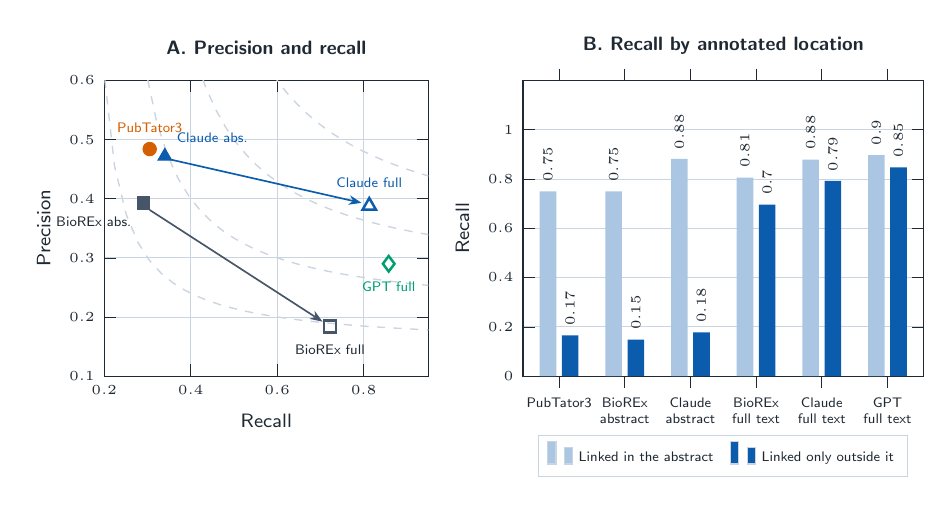
\begin{tikzpicture}
\begin{axis}[
  gdt, name=A,
  title={A. Precision and recall},
  width=0.47\linewidth, height=0.44\linewidth,
  xmin=0.2, xmax=0.95, ymin=0.1, ymax=0.6,
  xtick={0.2,0.4,0.6,0.8}, ytick={0.1,0.2,0.3,0.4,0.5,0.6},
  xlabel={Recall}, ylabel={Precision},
  clip mode=individual,
]
\foreach \F in {0.3,0.4,0.5,0.6} {
  \addplot[draw=rule, line width=0.5pt, dashed, domain=\F/2+0.02:0.95, samples=30, forget plot] {\F*x/(2*x-\F)};
}
\addplot[only marks, mark=*, mark size=2.4pt, color=pubtator] coordinates {(0.305,0.484)};
\addplot[only marks, mark=square*, mark size=2.2pt, color=stnf] coordinates {(0.291,0.393)};
\addplot[only marks, mark=square, mark size=2.2pt, line width=0.9pt, color=stnf] coordinates {(0.722,0.184)};
\addplot[only marks, mark=triangle*, mark size=2.8pt, color=ours] coordinates {(0.340,0.472)};
\addplot[only marks, mark=triangle, mark size=2.8pt, line width=0.9pt, color=ours] coordinates {(0.813,0.388)};
\addplot[only marks, mark=diamond, mark size=2.8pt, line width=0.9pt, color=gpt] coordinates {(0.858,0.290)};
\draw[-{Stealth[length=1.6mm]}, draw=ours, line width=0.6pt] (axis cs:0.355,0.466) -- (axis cs:0.795,0.393);
\draw[-{Stealth[length=1.6mm]}, draw=stnf, line width=0.6pt] (axis cs:0.305,0.381) -- (axis cs:0.705,0.192);
\node[font=\sffamily\tiny, text=pubtator, anchor=south] at (axis cs:0.305,0.495) {PubTator3};
\node[font=\sffamily\tiny, text=ink, anchor=north east] at (axis cs:0.285,0.385) {BioREx abs.};
\node[font=\sffamily\tiny, text=ink, anchor=north] at (axis cs:0.722,0.170) {BioREx full};
\node[font=\sffamily\tiny, text=ours, anchor=south west] at (axis cs:0.345,0.478) {Claude abs.};
\node[font=\sffamily\tiny, text=ours, anchor=south] at (axis cs:0.813,0.402) {Claude full};
\node[font=\sffamily\tiny, text=gpt, anchor=north] at (axis cs:0.858,0.275) {GPT full};
\end{axis}
\begin{axis}[
  gdt, at={(A.east)}, anchor=west, xshift=1.2cm,
  title={B. Recall by annotated location},
  ybar, bar width=6pt,
  width=0.55\linewidth, height=0.44\linewidth,
  ymin=0, ymax=1.2, ytick={0,0.2,0.4,0.6,0.8,1.0}, ylabel={Recall},
  symbolic x coords={pt,ba,ca,bf,cf,gf},
  xtick=data,
  xticklabels={PubTator3, BioREx\\abstract, Claude\\abstract, BioREx\\full text, Claude\\full text, GPT\\full text},
  xticklabel style={font=\sffamily\tiny, text=ink, align=center},
  xmajorgrids=false,
  enlarge x limits=0.11,
  legend style={font=\sffamily\tiny, text=ink, draw=rule, at={(0.5,-0.2)}, anchor=north, legend columns=2, /tikz/every even column/.append style={column sep=4pt}},
  nodes near coords={\pgfmathprintnumber[fixed, precision=2]{\pgfplotspointmeta}},
  nodes near coords style={font=\sffamily\tiny, text=ink, rotate=90, anchor=west},
]
\addplot[fill=ours!35, draw=none] coordinates {(pt,0.750) (ba,0.750) (ca,0.882) (bf,0.806) (cf,0.879) (gf,0.897)};
\addplot[fill=ours, draw=none] coordinates {(pt,0.165) (ba,0.148) (ca,0.177) (bf,0.696) (cf,0.792) (gf,0.847)};
\legend{Linked in the abstract, Linked only outside it}
\end{axis}
\end{tikzpicture}
}
\caption{\textbf{Full-text input raises recall most for the LLMs and BioREx; measured precision falls most for BioREx.} BioTriplex locked set, valid articles per system (Table~\ref{tab:main}). (A)~Precision and recall; arrows join abstract and full-text input for one system, and dashed curves are iso-F1 contours from 0.3 to 0.6. (B)~Recall on gold relations linked in the abstract and linked only outside it. PubTator3 relations derive from abstracts. Precision is computed against a non-exhaustive annotation.}
\label{fig:pr}
\end{figure}

\begin{table}[!htbp]
\centering\footnotesize
\caption{\textbf{Paired comparisons on BioTriplex separate input scope from method.} Differences (A minus B) on articles with valid results for both, with 95\% bootstrap intervals.}
\label{tab:pairs}
\resizebox{\linewidth}{!}{%
\begin{tabular}{@{}lcccc@{}}
\toprule
Comparison (A $-$ B) & Articles & $\Delta$ Precision & $\Delta$ Recall & $\Delta$ F1\\
\midrule
\multicolumn{5}{@{}l}{\emph{Same input, different method}}\\
Claude abstract $-$ PubTator3 & 28 & $-$0.017 [$-$0.178, 0.159] & +0.034 [$-$0.080, 0.173] & +0.019 [$-$0.093, 0.150]\\
Claude full $-$ BioREx full & 25 & +0.173 [0.087, 0.267] & +0.082 [$-$0.124, 0.267] & +0.193 [0.088, 0.292]\\
GPT full $-$ BioREx full & 27 & +0.097 [0.006, 0.199] & +0.134 [$-$0.054, 0.310] & +0.129 [0.012, 0.246]\\
Claude full $-$ RENET2 full & 25 & $-$0.007 [$-$0.185, 0.138] & +0.448 [0.230, 0.610] & +0.145 [$-$0.013, 0.291]\\
GPT full $-$ RENET2 full & 27 & $-$0.132 [$-$0.323, 0.036] & +0.520 [0.333, 0.655] & +0.058 [$-$0.134, 0.238]\\
\addlinespace
\multicolumn{5}{@{}l}{\emph{Same method, different input}}\\
Claude full $-$ Claude abstract & 25 & $-$0.117 [$-$0.355, 0.058] & +0.448 [0.299, 0.588] & +0.101 [$-$0.052, 0.254]\\
GPT full $-$ GPT abstract & 12 & $-$0.088 [$-$0.292, 0.061] & +0.581 [0.450, 0.689] & +0.141 [0.017, 0.251]\\
BioREx full $-$ BioREx abstract & 30 & $-$0.209 [$-$0.346, $-$0.105] & +0.430 [0.290, 0.583] & $-$0.042 [$-$0.162, 0.083]\\
RENET2 full $-$ RENET2 abstract & 30 & $-$0.173 [$-$0.318, $-$0.008] & +0.099 [$-$0.036, 0.244] & +0.022 [$-$0.092, 0.116]\\
\addlinespace
\multicolumn{5}{@{}l}{\emph{Reproduction check}}\\
BioREx abstract $-$ PubTator3 & 30 & $-$0.091 [$-$0.198, 0.005] & $-$0.013 [$-$0.110, 0.055] & $-$0.039 [$-$0.135, 0.029]\\
\bottomrule
\end{tabular}}
\end{table}

\subsection{Second BioTriplex Validation Batch}
The recall gain from full text recurred on the 49 further articles (Table~\ref{tab:batch2}). In the primary comparison, with failed articles counted as empty answers, Claude's full-text recall exceeded its abstract recall by 0.322 [0.133, 0.477] (0.632 vs 0.310). On the 35 articles with both inputs the difference was 0.518 [0.374, 0.626], and recall on relations linked only outside the abstract rose by 0.660 [0.500, 0.783]. BioREx rose by 0.508 [0.423, 0.578]. RENET2 did not change detectably (+0.015 [$-0.041$, 0.075]), which agrees with its smaller gain on the locked set.

Method comparisons use the 35 articles with valid Claude output, because a blocked article says nothing about extraction ability. On these articles, Claude's F1 exceeded RENET2's by 0.262 [0.148, 0.365] and BioREx's by 0.150 [0.104, 0.194]; its recall was far above RENET2's (+0.653 [0.465, 0.777]) and similar to BioREx's ($-0.008$ [$-0.108$, 0.071]). Counting failed articles as empty measures what a user of this hosted model receives, a question of availability. In that view the F1 differences remained above zero (+0.198 [0.075, 0.304] and +0.116 [0.043, 0.165]), and Claude's recall was 0.216 [0.076, 0.389] below BioREx's because 14 articles returned nothing. The F1 difference from RENET2, which spanned zero on the locked set, did not span zero here. Against PubTator3, Claude's F1 difference spanned zero on full text (+0.099 [$-0.028$, 0.209] on valid articles) and on abstracts (+0.032 [$-0.013$, 0.084]).

\begin{table}[!htbp]
\centering\footnotesize
\caption{\textbf{Full text raised recall again on 49 further BioTriplex articles, and failures lowered deployment recall.} One-to-one scoring, supported pairs; brackets give 95\% document-level bootstrap intervals for F1. Valid is the number of the 49 articles with a valid result; Deploy.\ F1 counts missing articles as empty answers. These articles were chosen after the locked results were known. $^{\ddagger}$PubTator3 relations derive from abstracts.}
\label{tab:batch2}
\begin{tabular}{@{}lccccc@{}}
\toprule
System & Valid & Precision & Recall & F1 & Deploy.\ F1\\
\midrule
PubTator3$^{\ddagger}$ & 49 & 0.495 & 0.304 & 0.377 [0.305, 0.454] & 0.377\\
BioREx, abstract & 49 & 0.423 & 0.340 & 0.377 [0.314, 0.441] & 0.377\\
RENET2, abstract & 49 & 0.471 & 0.195 & 0.275 [0.202, 0.350] & 0.275\\
Claude, abstract & 48 & 0.583 & 0.319 & 0.412 [0.335, 0.490] & 0.405\\
\addlinespace
BioREx, full text & 49 & 0.197 & 0.848 & 0.320 [0.256, 0.376] & 0.320\\
RENET2, full text & 49 & 0.272 & 0.210 & 0.237 [0.175, 0.304] & 0.237\\
Claude, full text & 35 & 0.332 & 0.829 & 0.474 [0.396, 0.541] & 0.435\\
\bottomrule
\end{tabular}
\end{table}

\subsection{Decomposing Apparent False Positives}
Claude's supported pairs outside the gold set fell mostly in the category of two gold entities without a linked relation, whereas BioREx's fell mostly in entity-scope categories (Fig.~\ref{fig:fp}A). On 25 shared articles, Claude reported 281 supported pairs and BioREx 456; 109 and 98 matched gold relations. Pairs with both entities in the gold set but no linked relation were similar in number (91 vs 89). BioREx had more pairs whose disease was not a BioTriplex disease (170 vs 44), whose gene or both entities were not gold entities (61 vs 26), and duplicates of a credited pair (38 vs 11).

The exploratory checks give concrete examples of these disagreements and do not correct precision (Table~\ref{tab:checks}, Fig.~\ref{fig:fp}B). In samples from the first category, the single annotator judged that the shown paragraphs state some relation for 33 of 35 Claude pairs across two sheets; in the mixed sheet both systems scored 13 of 15. This judgment is broader than BioTriplex's requirement for a relation phrase of a defined type, so these pairs are not shown to be annotation errors. In the out-of-scope disease category, 6 of 15 marked terms were judged not to be diseases for each system (for example \emph{mortality}, \emph{recurrence}, \emph{lung}, \emph{involvement}); a disease with a stated relation occurred in 9 of 15 Claude pairs and 6 of 15 BioREx pairs. On BioRED Dev, all 16 checked pairs supported only by the minimal prompt were judged to have a stated relation.

\begin{figure}[!htbp]
\centering
\resizebox{\linewidth}{!}{% Figure 4. Where full-text predictions fall against BioTriplex (A) and the blinded checks of two categories (B).
% A: 25 articles valid for both systems, experiments/biorex/README.md. B: experiments/biotriplex/precision_check,
% precision_compare and scope_check (result.json); V6 unannotated pairs pool both checks (33 of 35).
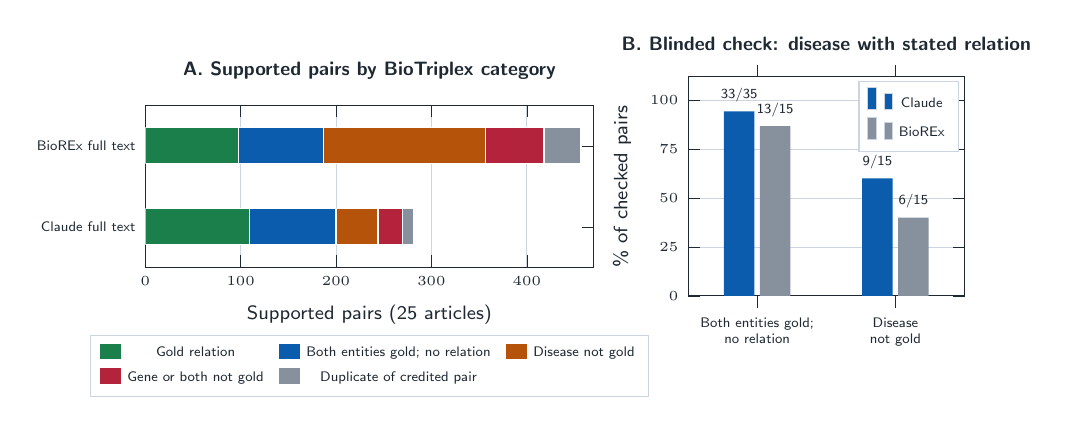
\begin{tikzpicture}
\begin{axis}[
  gdt, name=A,
  title={A. Supported pairs by BioTriplex category},
  xbar stacked, bar width=13pt,
  width=0.60\linewidth, height=0.30\linewidth,
  xmin=0, xmax=470, xtick={0,100,200,300,400}, xlabel={Supported pairs (25 articles)},
  symbolic y coords={BioREx,Claude},
  ytick=data, y dir=reverse,
  yticklabels={BioREx full text, Claude full text},
  yticklabel style={font=\sffamily\tiny, text=ink},
  ymajorgrids=false, enlarge y limits=0.5,
  legend style={font=\sffamily\tiny, text=ink, draw=rule, at={(0.5,-0.42)}, anchor=north, legend columns=3, /tikz/every even column/.append style={column sep=3pt}},
  reverse legend=false,
]
\addplot[fill=stsup, draw=white] coordinates {(98,BioREx) (109,Claude)};
\addplot[fill=ours, draw=white] coordinates {(89,BioREx) (91,Claude)};
\addplot[fill=stunc, draw=white] coordinates {(170,BioREx) (44,Claude)};
\addplot[fill=stneg, draw=white] coordinates {(61,BioREx) (26,Claude)};
\addplot[fill=stnf!65, draw=white] coordinates {(38,BioREx) (11,Claude)};
\legend{Gold relation, Both entities gold; no relation, Disease not gold, Gene or both not gold, Duplicate of credited pair}
\end{axis}
\begin{axis}[
  gdt, at={(A.east)}, anchor=west, xshift=1.2cm,
  title={B. Blinded check: disease with stated relation},
  ybar, bar width=11pt,
  width=0.42\linewidth, height=0.36\linewidth,
  ymin=0, ymax=112, ytick={0,25,50,75,100}, ylabel={\% of checked pairs},
  symbolic x coords={un,dis},
  xtick=data,
  xticklabels={Both entities gold;\\no relation, Disease\\not gold},
  xticklabel style={font=\sffamily\tiny, text=ink, align=center},
  xmajorgrids=false, enlarge x limits=0.5,
  legend style={font=\sffamily\tiny, text=ink, draw=rule, at={(0.98,0.98)}, anchor=north east},
  point meta=explicit symbolic,
  nodes near coords, nodes near coords style={font=\sffamily\tiny, text=ink},
]
\addplot[fill=ours, draw=none] coordinates {(un,94.3)[33/35] (dis,60.0)[9/15]};
\addplot[fill=stnf!65, draw=none] coordinates {(un,86.7)[13/15] (dis,40.0)[6/15]};
\legend{Claude, BioREx}
\end{axis}
\end{tikzpicture}
}
\caption{\textbf{The two systems differ mainly in entity-scope categories and duplicate pairs.} (A)~Supported pairs on the 25 BioTriplex articles valid for both systems, by external annotation category. (B)~Share of blindly checked pairs judged to involve a disease with a stated relation, by category, from one annotator; Claude's first bar pools two sheets.}
\label{fig:fp}
\end{figure}

\begin{table}[!htbp]
\centering\footnotesize
\caption{\textbf{Blinded single-annotator checks of pairs outside the gold sets.} Stated counts relation or hedged relation. Controls come from the gold annotation and were mixed in blind; agreement counts positives judged stated and negatives judged not stated. One control on the first BioTriplex sheet was left unanswered.}
\label{tab:checks}
\begin{tabularx}{\linewidth}{@{}Xlcc@{}}
\toprule
Sheet and category & System & Stated / checked & Control agreement\\
\midrule
BioRED Dev, supported only by the minimal prompt & Claude & 16 / 16 & 9 / 10\\
BioTriplex, entities gold, no relation (first sheet) & Claude & 20 / 20 & 6 / 9\\
BioTriplex, entities gold, no relation (mixed sheet) & Claude & 13 / 15 & 9 / 10\\
 & BioREx & 13 / 15 & \\
BioTriplex, disease not gold (mixed sheet; valid disease and stated) & Claude & 9 / 15 & 9 / 10\\
 & BioREx & 6 / 15 & \\
\bottomrule
\end{tabularx}
\end{table}

\subsection{Citation Sufficiency}
Every cited sentence ID resolved, but many citations did not name both entities. One cited sentence mentioned both for 139 of 241 supported pairs on BioRED (57.7\%) and 202 of 281 on BioTriplex (71.9\%). For 83 (34.4\%) and 71 (25.3\%), at least one entity had no mention in the cited sentences, usually the disease. Co-mention was more common for pairs overlapping a gold relation: 130 of 167 against 9 of 74 on BioRED, and 109 of 120 against 93 of 161 on BioTriplex.

In the blinded check, cited sentences alone were judged sufficient for a weighted 58.5\% [45.8, 70.9] of supported pairs on BioRED and 75.4\% [58.0, 89.1] on BioTriplex. Most of the remainder needed surrounding text (32.0\% and 19.0\%); 5.6\% on each corpus were judged unsupported, and 3.8\% on BioRED were hedged. With co-mention, 13 of 15 pairs were sufficient on both corpora; without it, 3 of 15 on BioRED and 7 of 15 on BioTriplex, so a missing co-mention flags a citation for review and does not show that it is wrong. All 5 unsupported pairs came from the stratum without co-mention; they included table cells giving a gene name and statistics, and a list of cytokines with no disease named. Of the 12 false-citation controls, 9 were judged unsupported, 1 hedged, 1 in need of context, and 1 sufficient. These controls are easy because one entity is absent, so they exclude gross acceptance only.

\subsection{Status Labels and BioRED Error Profile}
Non-binary statuses tracked graded gold labels on the small sets available. On EU-ADR, all 3 NA pairs were labelled \st{explicit\_negative} by both prompts, whereas PubTator3 predicted one as positive. On RENET2, 3 of the 202 minimal-prompt supported pairs outside the gold set contradicted a tool-assigned negative label; 131 had never been labelled. On BioRED Dev+Test, the minimal prompt missed 232 gold relations: 122 involved an endpoint outside its entities (65 diseases not recorded, 34 recorded as symptoms, 23 genes not recorded), 84 were judged non-supported (45 \st{not\_found}, 36 \st{uncertain}, 3 \st{explicit\_negative}), and 26 had a supported pair credited to another gold relation. Of its 125 extra pairs, 100 involved two gold concepts without a BioRED relation.

\subsection{Failures and Cost}
Failures of the minimal prompt were dominated by the provider's safety filter. After one retry, 2 of 100 BioRED Test abstracts, 6 of 100 EU-ADR abstracts, 7 of 40 RENET2 articles, and 5 of 30 BioTriplex full texts had no valid result. On BioTriplex, 4 articles were blocked in both attempts: two on pathogen challenge or infection, one on immune tolerance in arthritis-prone mice, and one on a muscular dystrophy model. GPT-6.1 Sol completed those 4. Blocking was not fixed to a document: one BioRED abstract was blocked in one run and completed in another. On the second BioTriplex batch, 17 of 49 full texts failed at first; one retry recovered 3, and the remaining 14 (29\%) all ended in a safety flag or refusal, against 1 of 49 abstracts. We did not probe the cause. Decision-card runs on BioRED, EU-ADR, and RENET2, made earlier, had no such failures; we cannot attribute this to the prompt because provider filters may change over time. Including repair calls at list API prices, the minimal prompt cost USD 0.072 per BioRED abstract, USD 0.091 per EU-ADR abstract, USD 0.30 per RENET2 article, and USD 0.40 per BioTriplex full text (mean 66\,s). BioREx ran on CPU in about 10 minutes for the 30 articles with no API cost.

%% ===================================================================
\section{Discussion}

\subsection{Input Scope and Coverage}
On abstracts, a 108-word prompt performed in the range of a supervised system trained on annotations from the same corpus family, and paired differences spanned zero on three corpora. On full text, recall more than doubled for both LLMs and for BioREx, so the coverage gain is not specific to LLMs. It is not automatic either: RENET2 gained less, possibly because it was trained on truncated texts and reads a limited number of sentences, or because its labels favour fewer pairs. The practical consequence for resources built from abstracts is direct: about three quarters of BioTriplex relations are annotated only outside the abstract, and abstract-level extraction reached 0.15--0.18 recall on them.

\subsection{Reading the Comparisons with Supervised Models}
The two supervised comparators sit at different points of a precision--recall trade-off, and neither is a ceiling for supervised methods. RENET2, trained on full text, matched Claude's measured precision with less than half its recall, so the LLM's difference from a full-text-trained model lies in recall, and the F1 differences were not distinguishable. RENET2's training labels were built from tool-proposed candidates on truncated texts, and BioTriplex annotates differently, so this comparison also mixes model and annotation style.

The BioREx comparison answers a narrow question: how an off-the-shelf pipeline trained on abstracts and transferred paragraph by paragraph compares with zero-shot LLMs under one scoring protocol. It does not show that LLMs judge relations better than supervised methods. The two systems differ little in pairs of gold entities without a linked relation (91 vs 89); most of the difference lies in out-of-scope entities and duplicates. A plausible mechanism is upstream of relation classification: the PubTator3 entity layer marks clinical outcomes, anatomical terms, and processes as diseases in body text, BioREx relates them per paragraph, and identifiers split entities. RENET2 used the same entities and reported far fewer pairs, which shows that the entity layer alone does not determine the outcome. Because BioTriplex defines the entity scope in this comparison, a pair outside it is not necessarily wrong. Entity scope and merging may deserve as much attention as relation classification when evaluating full-text pipelines.

\subsection{What the Card Ablation Shows}
This decision card was written to protect precision, and on BioRED and EU-ADR it lowered recall without a detectable precision gain. This is a finding about one prompt design. The ablation changed many rules and the length together, and the guideline variants were two single Dev runs on abstracts, so we cannot say which rule is responsible or whether detailed rules help or harm in general. Practically, a rule document written for one purpose should be tested against the target annotation before use. Reason-code routing partly recovers the loss after the fact without model calls. Format reliability, often credited to detailed prompts, was obtained here with deterministic pre-processing.

\subsection{Reading Benchmark Precision}
Precision against selective gold sets measures agreement with an annotation protocol, which can differ from correctness. RENET2 and BioTriplex precision for the LLMs was 0.22--0.39, and our exploratory checks show that some pairs outside these gold sets have a stated relation in the text. They do not establish how many, or that the gold sets are deficient. These gold sets remain the common reference for comparing systems, so all reported metrics use them. One-to-one matching also matters: many-to-one credit overstated precision substantially in our own earlier results.

\subsection{Implications for Curation}
The results support a division of labour. An abstract-level resource remains inexpensive and precise within its scope; full-text LLM extraction adds coverage and citations at about USD 0.40 per article, with the expectation that curators review output. Stored statuses and source labels allow different thresholds from one run. We make no claim about curation quality or efficiency, which require a user study. Cascades that verify supervised candidates~\cite{song2026core,adam2025traceable} are a natural extension, and safety-filter blocking of ordinary biomedical papers argues for a fallback model: on the second batch it lowered Claude's recall from 0.829 on valid articles to 0.632 on all articles.

\subsection{Limitations}\label{sec:limitations}
Seven limitations bound these conclusions. First, all blinded checks used one annotator who knew the hypotheses, with 15--30 pairs per cell; control agreement was 6 of 9 on one sheet, the annotator's criterion was broader than BioTriplex's requirement for a typed relation phrase, and categories such as gene-not-gold pairs were not checked. Second, the validator verifies verbatim entity matches and sentence-ID resolution, not that a cited sentence semantically supports a relation; the citation check covers 60 pairs from the minimal prompt with Claude, judged by that one annotator, and agreement of the source label with BioTriplex does not validate the citations. Third, the locked BioTriplex set is small (25--30 valid articles) and the second batch was chosen after its results were known and lacks a second LLM, its annotation comes mainly from one annotator, entity merging is our own rule, and the GPT abstract run stopped at 13 of 30 articles when API credits ran out. Fourth, neither supervised model was trained on BioTriplex: BioREx was neither retrained nor tuned for full text, RENET2 was run with default settings and our sentence splitter under a current PyTorch version, both use PubTator3 entities while LLMs select their own, and our task collapses relation types, so results are not comparable with published BioTriplex or BioCreative numbers. Fifth, the minimal prompt was chosen after BioRED Test results were seen; the card was not tested on BioTriplex; and neither rule content nor prompt length was isolated, so the prompt results compare specific versions. Prompt and input effects were measured on different corpora and cannot be ranked against each other. Sixth, missing documents may not be random: we could not determine what triggers safety-filter blocks, so valid-only metrics may not transfer to the blocked documents, and the failure rate differed between the two BioTriplex batches (13\% and 29\%). Seventh, both LLMs are proprietary and subject to change, benchmark texts may occur in pretraining data, entities are not normalized to identifiers, and most configurations ran once; we archive prompts, outputs, and scripts to support reproduction.

%% ===================================================================
\section{Conclusions}
A zero-shot pipeline with a short task prompt, sentence-ID citations, and deterministic validation performed in the range of PubTator3 on abstract-level input (F1 0.614 vs 0.680 on BioRED Test; 0.395 vs 0.377 on BioTriplex abstracts) while attaching sentence citations and status labels. One detailed decision card reduced F1 on BioRED by lowering recall. On a locked full-text set, reading the article raised recall from 0.366 to 0.813 for Claude Opus 5.5, with comparable gains for GPT-6.1 Sol and BioREx and a smaller change for RENET2, so input scope matters but its benefit depends on the system. On 49 further articles the recall gain recurred for Claude and BioREx and not for RENET2, while safety filters left 29\% of full texts without a Claude result. Against abstract-trained BioREx on the same paragraphs, both LLMs had higher F1 on the articles with valid output, with most of the difference in entity scope and duplicates; against full-text-trained RENET2, recall was higher, and F1 was not distinguishable on the locked set and higher on the further articles. In a single-annotator check, cited sentences alone were sufficient for 58.5\% of supported pairs on BioRED and 75.4\% on BioTriplex, so citations direct review and do not replace it. Future work should add independent dual annotation, repeat the citation check with a second annotator, retrain supervised models on full text, normalize entities, evaluate open-weight models, and test verification cascades and curator workflows.

%% ===================================================================
\section*{CRediT authorship contribution statement}
\todo{to be agreed with co-authors}

\section*{Declaration of competing interest}
\todo{to complete}

\section*{Data and code availability}
Code, prompts, raw model outputs and scoring scripts will be released at \todo{repository URL}. EU-ADR, RENET2, and BioTriplex texts are not redistributed; preparation scripts are provided.

\section*{Declaration of generative AI use}
\todo{Required by the publisher. Describe the use of AI tools in drafting this manuscript; check the current Elsevier wording.}

\section*{Acknowledgements}
\todo{funding and acknowledgements}

\bibliographystyle{elsarticle-num}
\bibliography{refs}

\end{document}
